\documentclass[a4paper]{article}

%% Language and font encodings
\usepackage[english]{babel}
\usepackage[utf8x]{inputenc}
\usepackage[T1]{fontenc}

%% Sets page size and margins
\usepackage[a4paper,top=3cm,bottom=2cm,left=3cm,right=3cm,marginparwidth=1.75cm]{geometry}

%% Useful packages
\usepackage{grffile}
\usepackage{listings}
\usepackage{algorithm}
\usepackage[noend]{algpseudocode}
\usepackage{float}
\usepackage{amsmath,bm,mathrsfs}
\usepackage{amsthm,amssymb}
\usepackage{graphicx}
%\usepackage[draft]{graphicx}
\usepackage[colorinlistoftodos]{todonotes}
\usepackage[colorlinks=true, allcolors=blue]{hyperref}

%% Operators
\newcommand{\R}{\mathcal{R}}
\newcommand{\RR}{\mathbb{R}}
\newcommand{\N}{\mathbb{N}}
\newcommand{\G}{\mathcal{G}}
\newcommand{\V}{\mathcal{V}}
\newcommand{\E}{\mathcal{E}}
\newcommand{\La}{\mathcal{L}}
\newcommand{\UR}{U_{\mathcal{R}}}
\newcommand{\vv}{\mathit{v}}
\renewcommand{\l}{\ell}

\theoremstyle{definition}
\newtheorem*{definition}{Definition}
\newtheorem*{thm}{Theorem}

\title{Notes}

\begin{document}
\maketitle

\newpage


\section{Things to fix:}
\begin{enumerate}
\item (fixed) Undefined function 'findpeaks' for input
arguments of type 'double'.

Error in mcsfb\_design\_filter\_bank\_no\_fourier
(line 31)
    [~, idx] = findpeaks(inverted); 
    
\item (fixed) Warning: Matrix is close to singular or badly scaled (Reconstruction using eigenvalue and eigenvectors)


\item filter design function - does not perform well

\end{enumerate}

\section{Notations}
Consider a weighted, undirected graph $\G = \{ \V, \E, W\}$, where $\V$ is the set of $N$ vertices, $\E$ is the set of edges and $W$ is the associated weighted adjacency matrix. Let $D$ be the diagonal matrix of vertex degrees. Denote $\La$ as the graph Laplacian, where $\La = D-W$. Since $\La$ is real, symmetric and semi-definite, we can diagonalize it as $\La =U\Lambda U^*$, where $\Lambda$ is the diagonal matrix of its real eigenvalues $\lambda_0, \lambda_1,\cdots, \lambda_{N-1}$ and the columns $u_0, u_1 \cdots u_{N-1}$ of $U$ are corresponding orthonormal eigenvectors of $\La$. We use $\UR$ to denote the submatrix formed by taking the columns of $U$ associated with the Laplacian eigenvalues indexed by $\mathcal{R} \subseteq \{0,1,\cdots,N-1\}$. And we use $U_{\mathcal{S},\mathcal{R}}$ to denote the submatrix formed by taking the rows of $U_{\mathcal{R}}$ associated with the vertices indexed by the set $\mathcal{S} \subseteq \{1,2,\cdots, N\}$. For $i \in \{1,\cdots,n\}$, $\bm{\delta_i} \in \RR^n$ denotes the $i$th column of the identity matrix $I \in \RR^{n\times n}.$
We consider graph signals $f \in \RR^N$ residing on a graph $\G$. A signal $f \in \RR^n$ defined on the nodes of the graph $\G$ is $\R$-concentrated if $f \in \text{span}(U_{\R})$. The graph Fourier transform of a signal is $\hat{f} = U*f$ and $\hat{g}(\La) f = U\hat{g}(\Lambda)U*f$ filters a graph signal by $\hat{g}(\cdot)$. Signal $r\in \RR^N$ is a random vector such that each entry is randomly draw from a standard gaussian distribution.

\medskip

\section{Definitions}
%\begin{definition}
%A signal $\bm{x} \in \RR^n$ defined on the nodes of the graph $\G$ is $k$-bandlimited with $k \in \N^+$ if $\bm{x} \in \text{span}(U_{\R})$ and $|\R| = k$.
%\end{definition}

\begin{definition}
A signal $\bm{f} \in \RR^n$ defined on the nodes of the graph $\G$ is $\R$-concentrated if $\bm{f} \in \text{span}(U_{\R})$.
\end{definition}

\begin{definition}
Let $\bm{p} \in \RR^{n}$ represent a sampling distribution on $\{1,2,\cdots n\}$. The graph weighted coherence of order $|\R| $ for the pair $(\G, \bm{p})$ is
$$ \vv^k_{\bm{p}} = \underset{1\leq i\leq n}{\text{ max }} \{\bm{p_i}^{-1/2} ||U_{\R}^T \bm{\delta_i} ||_2\}$$

\end{definition}

\section{Theorems}
\begin{thm}[Orthogonality Proof]

Let $\{\R_1, \R_2, \cdots, \R_M\}$ be $M$ partitions of the graph Laplacian eigenvalue indices $\{0, 1, \cdots,  N \}$ and $\{g_1, g_2, \cdots, g_M \}$ be filters defined on each of the $M$ bands. Then, the subspace spanned by $g_i(\La)$ is orthogonal to the subspace spanned by $g_j(\La)$ for $i \neq j$

\end{thm}

\begin{proof}


Notice that the $(i,j)$ entry of matrix $g(\La)$ can be represented as 

$$g(\La) (i,j) = [Ug(\Lambda)U^T] (i,j) = \sum_{k = 1}^{N} g(\lambda_k) U_k(i) U_k(j)$$

Now consider two filters $g_1$ and $g_2$. To show that two subspaces spanned are orthogonal, we show that the dot product of any two vectors is 0.
\begin{align*}
g_1(\La)(,k) \cdot g_2(\La)(,l)&=\ \  \sum_{j = 1}^{N} [\sum_{k = 1}^{N} g_1(\lambda_k) U_k(i) U_k(j) )( \sum_{l = 1}^{N} g_2(\lambda_l) U_l(i) U_l(j)) ] \\
& = \sum_{k = 1}^{N} \sum_{l = 1}^{N} g_1(\lambda_k) g_2(\lambda_l)  U_k(i) U_l(i) ( \sum_{j = 1}^{N}  U_k(j)  U_l(j))  \\
& = \sum_{k = 1}^{N} g_1(\lambda_k) g_2(\lambda_k)  U_k(i) U_k(i) ( \sum_{j = 1}^{N}  U_k(j)  U_k(j)) 
\end{align*}

Notice that $g_1(\lambda_k) g_2(\lambda_k)$ is always equal to $0$, since $g_1$ and $g_2$ are defined on disjoint sets of Laplacian eigenvalues.   

\end{proof}



%\begin{proof}

%$$g_1(\La) = Ug_1(\Lambda)U^T$$

%$$g_2(\La) = Ug_2(\Lambda)U^T$$

%Notice that $g_1(\lambda_k) g_2(\lambda_k)$ is always equal to $0$, since $g_1$ and $g_2$ are defined on disjoint sets of Laplacian eigenvalues.  
%\end{proof}
%\end{comment}


\newpage

\section{Abstract}
     We investigate an $M$-channel critically sampled filter bank for graph signals where each of the $M$ filters is supported on a different subband of the graph Laplacian spectrum. For analysis, on each subband, the graph signal is filtered using efficient polynomial approximation methods and then downsampled on a corresponding set of vertices chosen via non-uniform random sampling. We use an efficient decoder derived from the non-uniform sampling distribution to reconstruct the filtered signals on each band from their samples. We leverage an approximation of the spectral density function of the graph Laplacian to both approximate the number of eigenvalues in each band and design the filter bank to be more amenable to polynomial approximation, in order to reduce the resulting reconstruction error. We empirically explore the joint vertex-frequency localization of the dictionary atoms, the sparsity of the analysis coefficients, and the ability of the proposed transform to compress piecewise-smooth graph signals. 



\section{Filter Bank Design}

In this section, we construct a scalable $M$-channel critically sampled filter bank where each of the $M$ filters is supported on a different subband of the graph Laplacian spectrum. The ideal filter bank design requires full eigendecomposition the graph Laplacian, which takes $\Theta(N^3)$ operations with regard to the size of the graph. In order to circumvent these expensive computations, we estimate the spectral density function of the graph Laplacian and then adopt it to efficiently design the the filter bank. The filters are then stored and applied using the polynomial approximation methods discussed in \cite{hammond2011wavelets, shuman_DCOSS_2011}. 

\subsection{Estimate Spectral Density Function}

Various methods have been proposed by past literature to estimate the spectral density functions, including the spectrum slicing method\cite{hammond2011wavelets,shuman_DCOSS_2011}, the Lanczos algorithm, the kernel polynomial method \cite{approximating spectral densities of large matrices} and etc. We direct readers to \cite{} for more information. Here, we give a brief overview of the KPM, which is the method we use in our implementation.

Given a filter $\hat{g}(\cdot)$, we notice that $\hat{g}(\La)$ is a diagonal matrix, where $\hat{g}(\La)_{i,i} = 1$ if the $i$th eigenvalue is covered by the filter and $\hat{g}(\La)_{i,i} = 0$, otherwise. By computing the trace of $\hat{g}(\La)$, which is the sum of the diagonal, we obtain the number of eigenvalues in the band specified by $\hat{g}(\cdot)$. This method scales linearly with regard to the size of the graph. In practice, the trace can be approximated using the following fact:

$$tr(\hat{g}(\La)) = E[r^T\hat{g}(\La)r] \propto \frac{1}{I}\sum_{i =1}^{I} (r^{i})^T\hat{g}(\La)r^{i}$$

We pick $n$ linearly spaced points $(x_1, \cdots, x_n)$ over the entire spectrum. Using the trace estimator, we can easily compute the number of eigenvalues, $y_i$, in $[0, x_i]$ for $0\leq i \leq n$. Finally, we use the monotonic cubic polynomial interpolation method with interpolation points $\{(x_i, y_i)\}_{0\leq i \leq n}$ to form a smooth function that estimates the cumulative spectral density function.


\subsection{Fast Filtering}

Recall that $\hat{g}(\cdot)$ filters a signal $f$ by $\hat{g}(\La) f = U\hat{g}(\Lambda)U*f$, where $\hat{g}(\Lambda) = (\hat{g}(\lambda_1), \cdots, \hat{g}(\lambda_n))^T.$  To avoid the computation of $U$ and $\Lambda$ in the filtering process, one common approach is to approximate the exact filter $\hat{g}(\cdot)$ by a polynomial function:

$$\hat{g} = \sum_{k = 0}^{\infty} c_kT_k.$$

In our implementation, we allow two different polynoial approximation methods: Chebyshev and Jackson-Chebyshev approximations. For example, the truncated Chebyshev polynomial approximation can be represented as 

$$\hat{g}(\La)f = \frac{1}{2}c_0f + \sum_{k=1}^{\infty} c_k \bar{T}_k(\La)f \propto \frac{1}{2}c_0f + \sum_{k=1}^{K} c_k \bar{T}_k(\La)f$$ and each $\bar{T}_k(\La)f$ can be efficiently computed recursively from $\bar{T}_{k-1}(\La)f$ and $\bar{T}_{k-2}(\La)f$. 

Jackson-Chebyshev method adds in one more damping multiplier, $g_j^K$, to alleviate the Gibbs oscillations near the boundaries:
$$\hat{g}(\La)f \propto \frac{1}{2}g_0^Kc_0f + \sum_{k=1}^{K} g_k^Kc_k \bar{T}_k(\La)f.$$

For the scalable filter bank, instead of storing the exact filters, we store the coefficients of Chebyshev or Jackson-Chebyshev polynomial approximations and the filters will be applied to any given signal accordingly. See \cite{shuman2013spectrum}, \cite{Druskin and Knizhnerman} for more information on polynomial approximation and \cite{fast filtering} for more fast filtering techniques. Two examples of polynomial approximated filters using Jackson-Chebyshev coefficients are shown in the figure below.
 
 \begin{figure}[h]
 \centering
 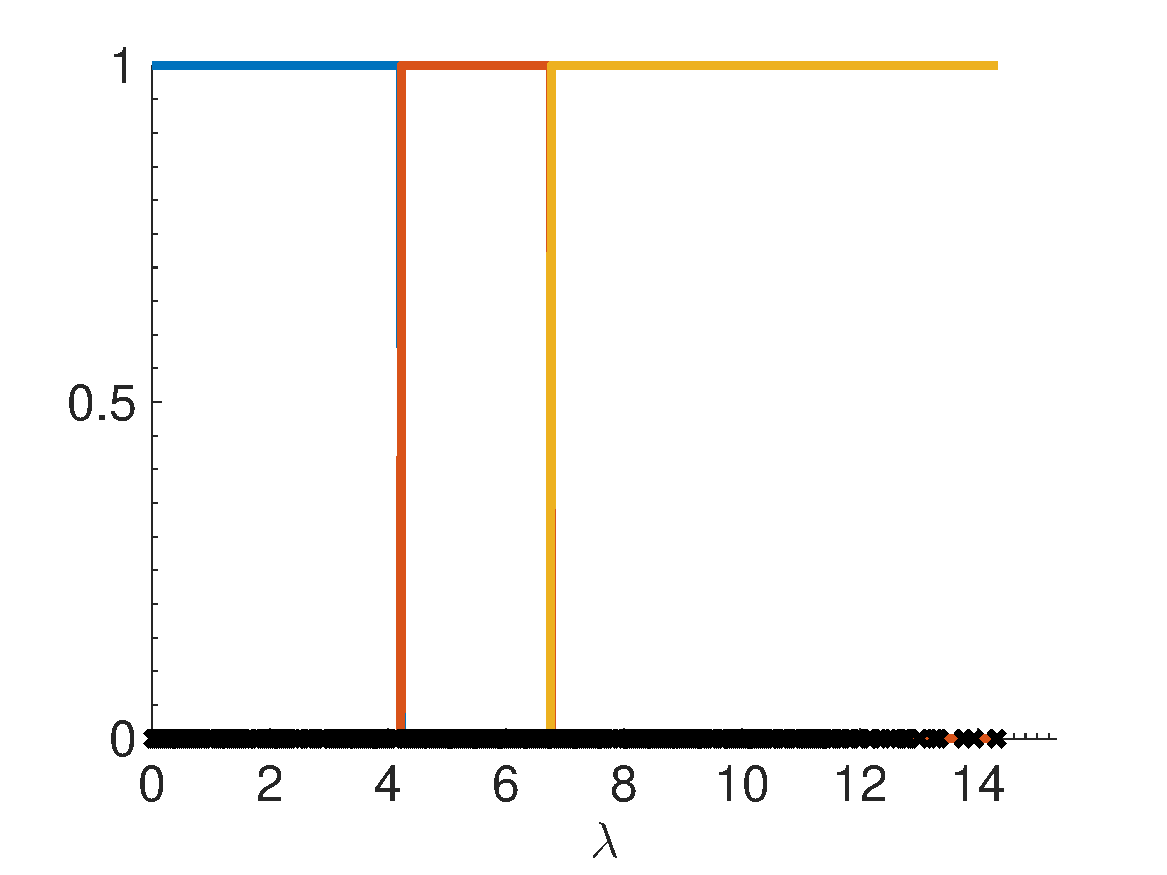
\includegraphics[width = 5cm]{ideal filter bank sensor.pdf}
 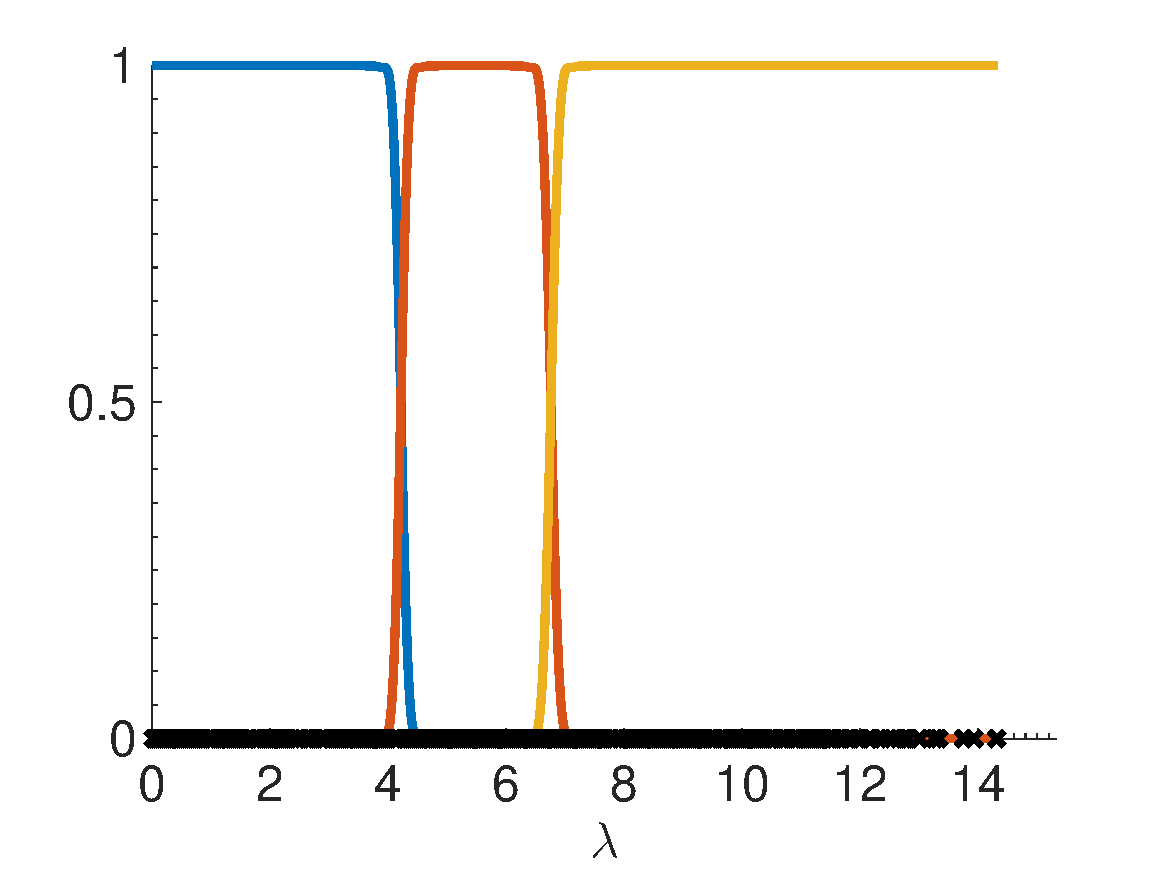
\includegraphics[width = 5cm]{approx filter bank sensor.pdf}
 
 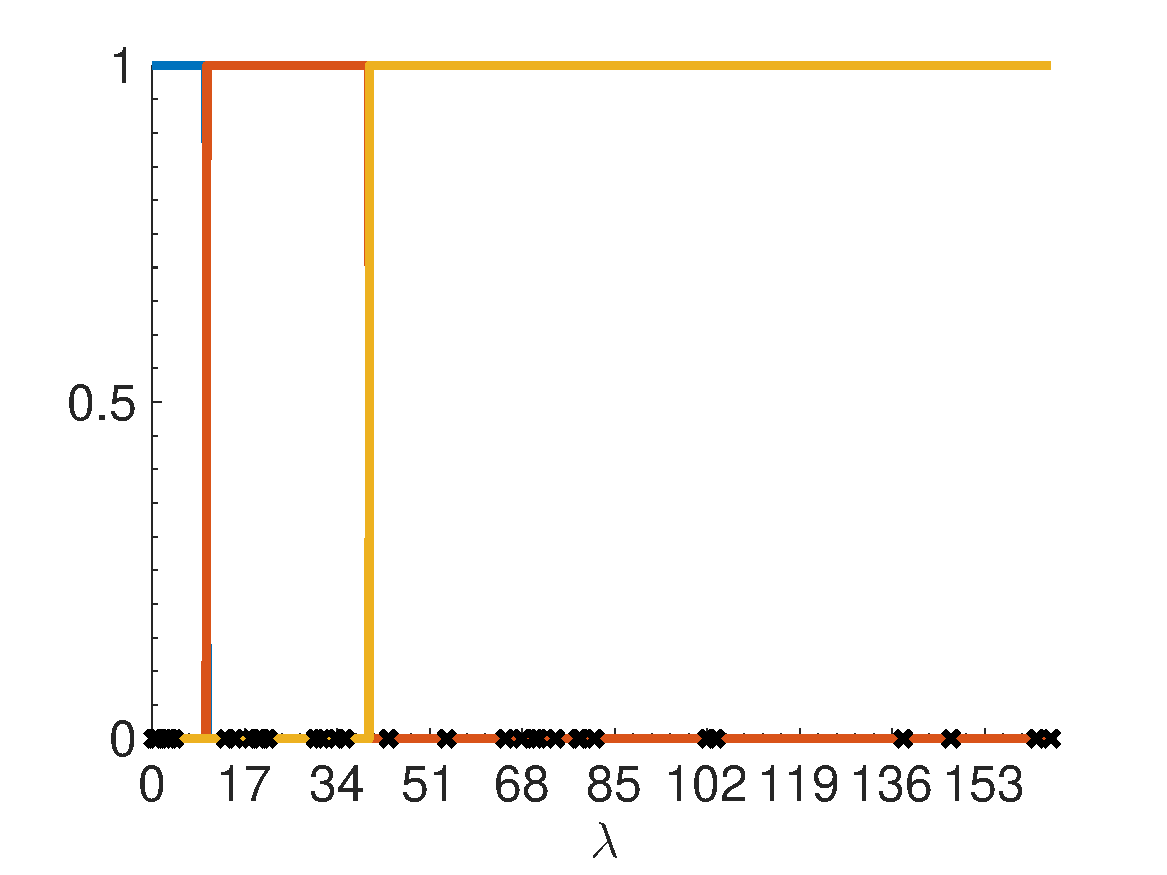
\includegraphics[width = 5cm]{ideal filter bank net25.pdf}
 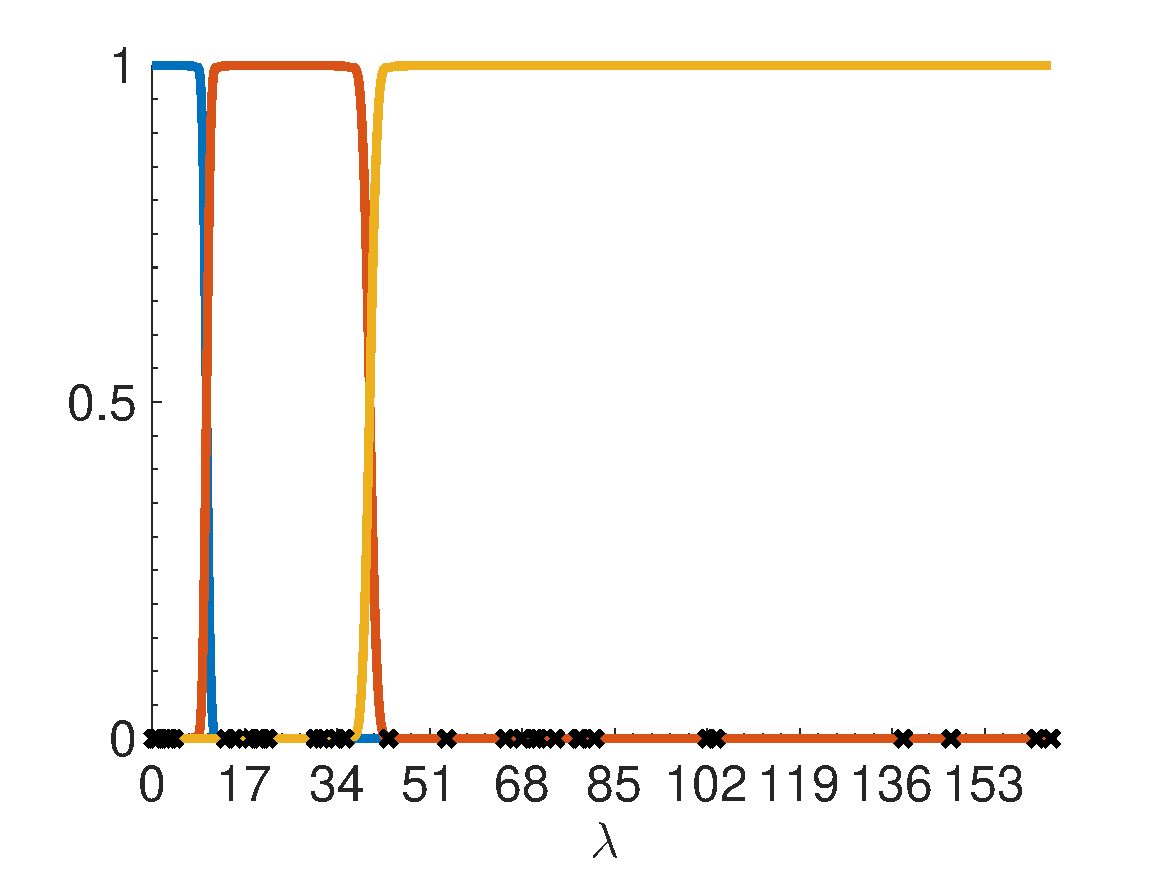
\includegraphics[width = 5cm]{approx filter bank net25.pdf}
 
 \caption{The first two examples are ideal and approximated filter banks for a more evenly distributed spectrum. The other two examples are for a graph with noticeable spectral gaps.}
 \end{figure}


\subsubsection{Adjust Band Ends to Minimize Approximation Error}
When selecting the band ends for each of the $M$ ideal filters, we consider two factors: spectrum-adaptation and band spacing method. In our implementation, the filter bank can be either spectrum-adapted or not, and it can be either evenly spaced or logarithmic spaced.

Without a full knowledge of the spectrum of the graph Laplacian, we cannot pick the band ends the way as we do for ideal filter banks. We first pick the band ends based on the approximated spectral functions. While satisfying the spectrum-adaptation and spacing requirements, we shift our initial choices of band ends in a small interval in order to reduce the resulting reconstruction error.

Consider the exact filter $\hat{g}$ and the polynomial approximated filter $\hat{h}(\La)$. If $K$ is the order of the polynomial approximation, the filtering error is 
$$||\hat{g}(\La) - \hat{h}(\La)|| = \text{max}_{l = 0,\cdots,n} |g(\lambda_l) - h(\lambda_l)| \leq \text{sup}_{\lambda \in [0, \lambda_{max}]} |g(\lambda) - h(\lambda)| = \Omega(\rho^{-K})$$
Notice that for Chebyshev and Jackson-Chebyshev approximations, the filtering error is always clustered around band boundaries (figure 1). If the boundaries are set in spectral gaps, i.e. there are no or very few eigenvalues around it, the approximated filters will not affect the filtering accuracy too much, thus leading to a small reconstruction error.  

Our approach to locate the spectral gaps is simply to find the minimum of the probability distribution of Laplacian eigenvalues over a specified interval. Let the $w$ be the width of the adjustment interval. For an initial choice of the band end $m \in [\tau, \tau+w]$, we intend to find $\tau$ such that the cumulative density function $F(\tau+w)-F(w)$ is minimized. That is, we want to minimize the probability of eigenvalues existing in the interval $[\tau, \tau+w]$. When $w$ is small, it is equivalent to find the $\tau$ such that the probability distribution of the Laplacian eigenvalues $p(\tau)$ is minimized. This process is illustrated in the figure below.


\begin{figure}[h]
\centering
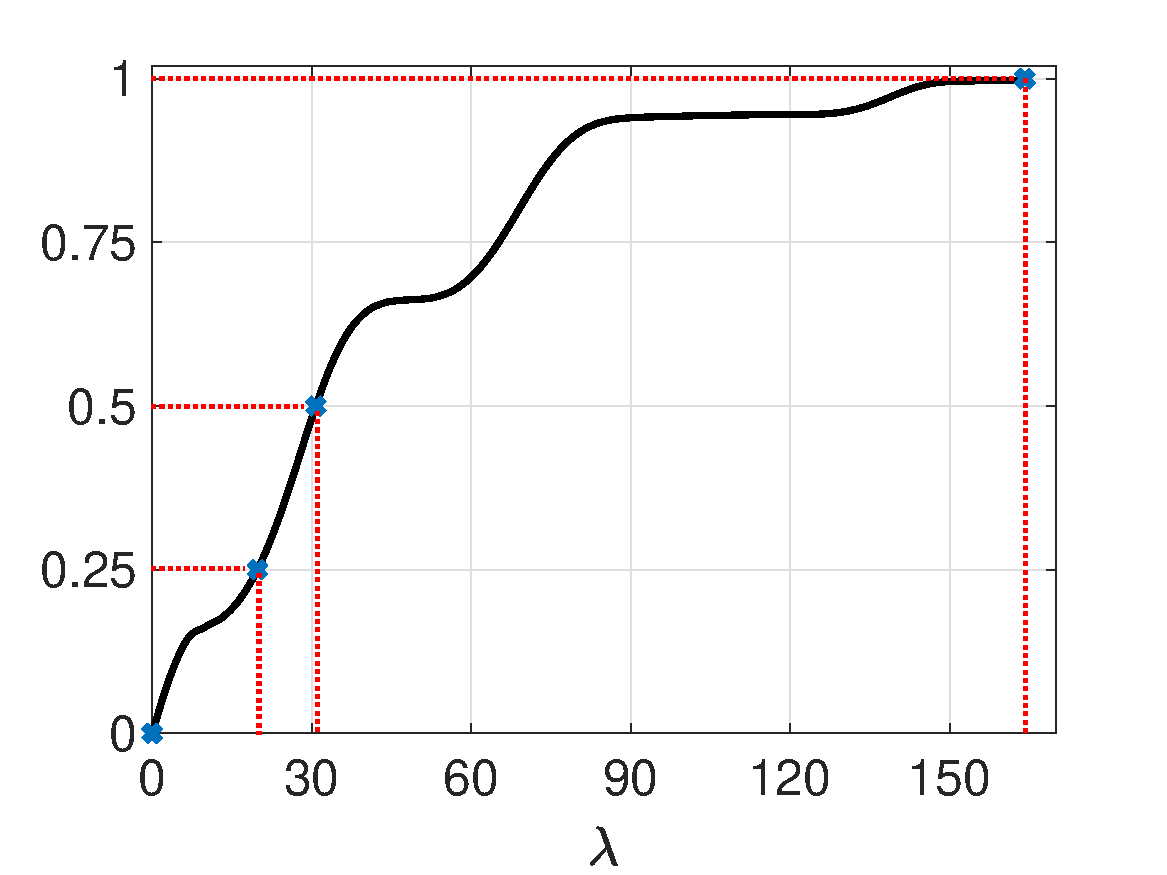
\includegraphics[width = 5cm]{cdf.pdf}
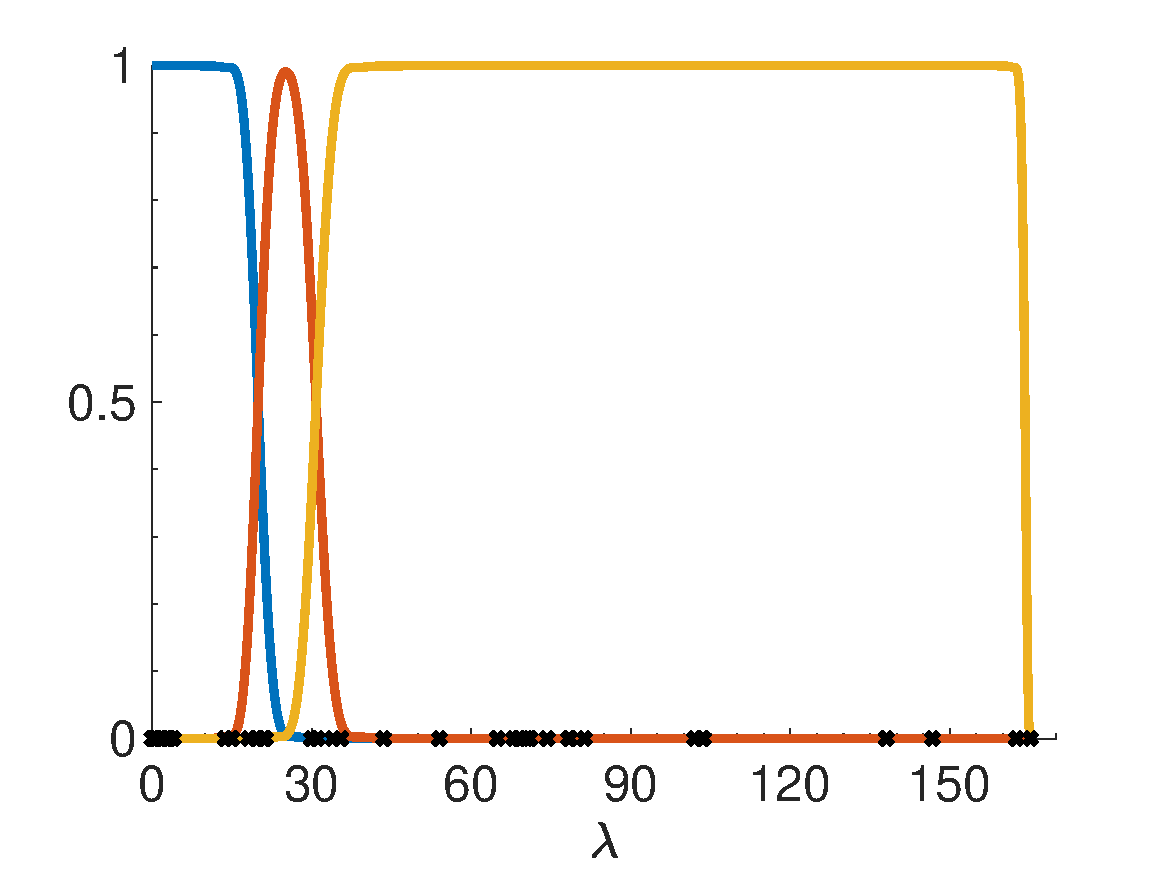
\includegraphics[width = 5cm]{original filter bank.pdf}

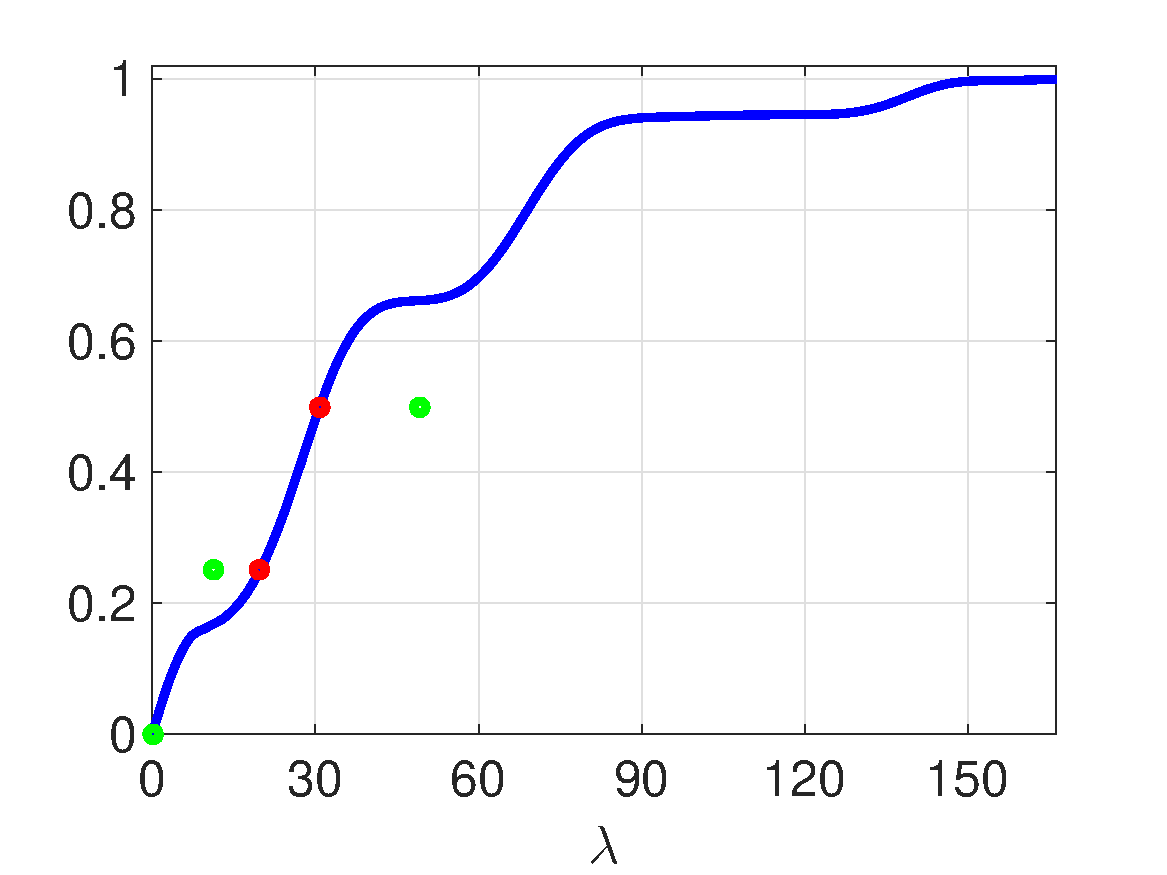
\includegraphics[width = 5cm]{shifted ends.pdf}
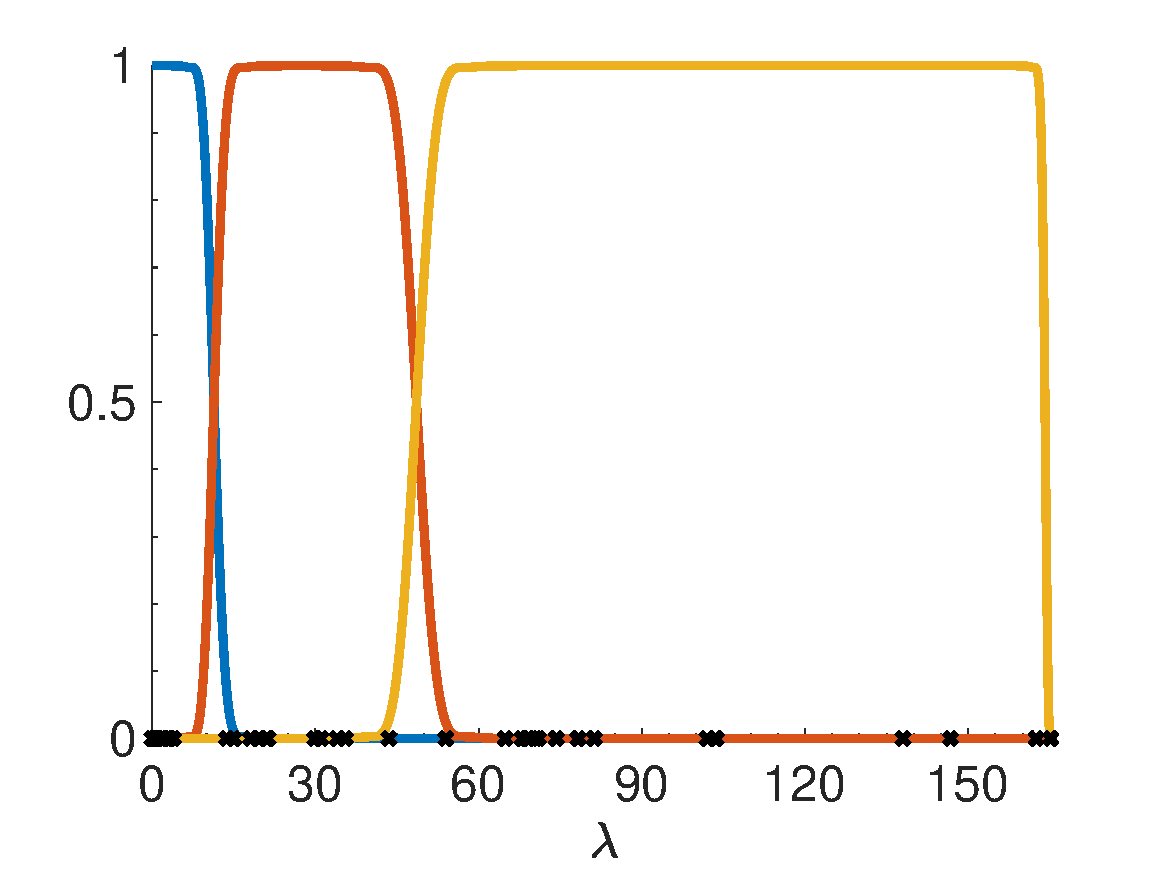
\includegraphics[width = 5cm]{updated filter bank.pdf}

\caption{(a) shows the initial band end choices for a a spectrum-adapted and logarithmic spaced filter bank of 3 filters. (b) is the approximated filter bank based on the initial choices. In (c), the green dots indicate the shifted band ends and (d) is the update filter bank.}
\end{figure}




\iffalse
\begin{figure}[h]
\centering
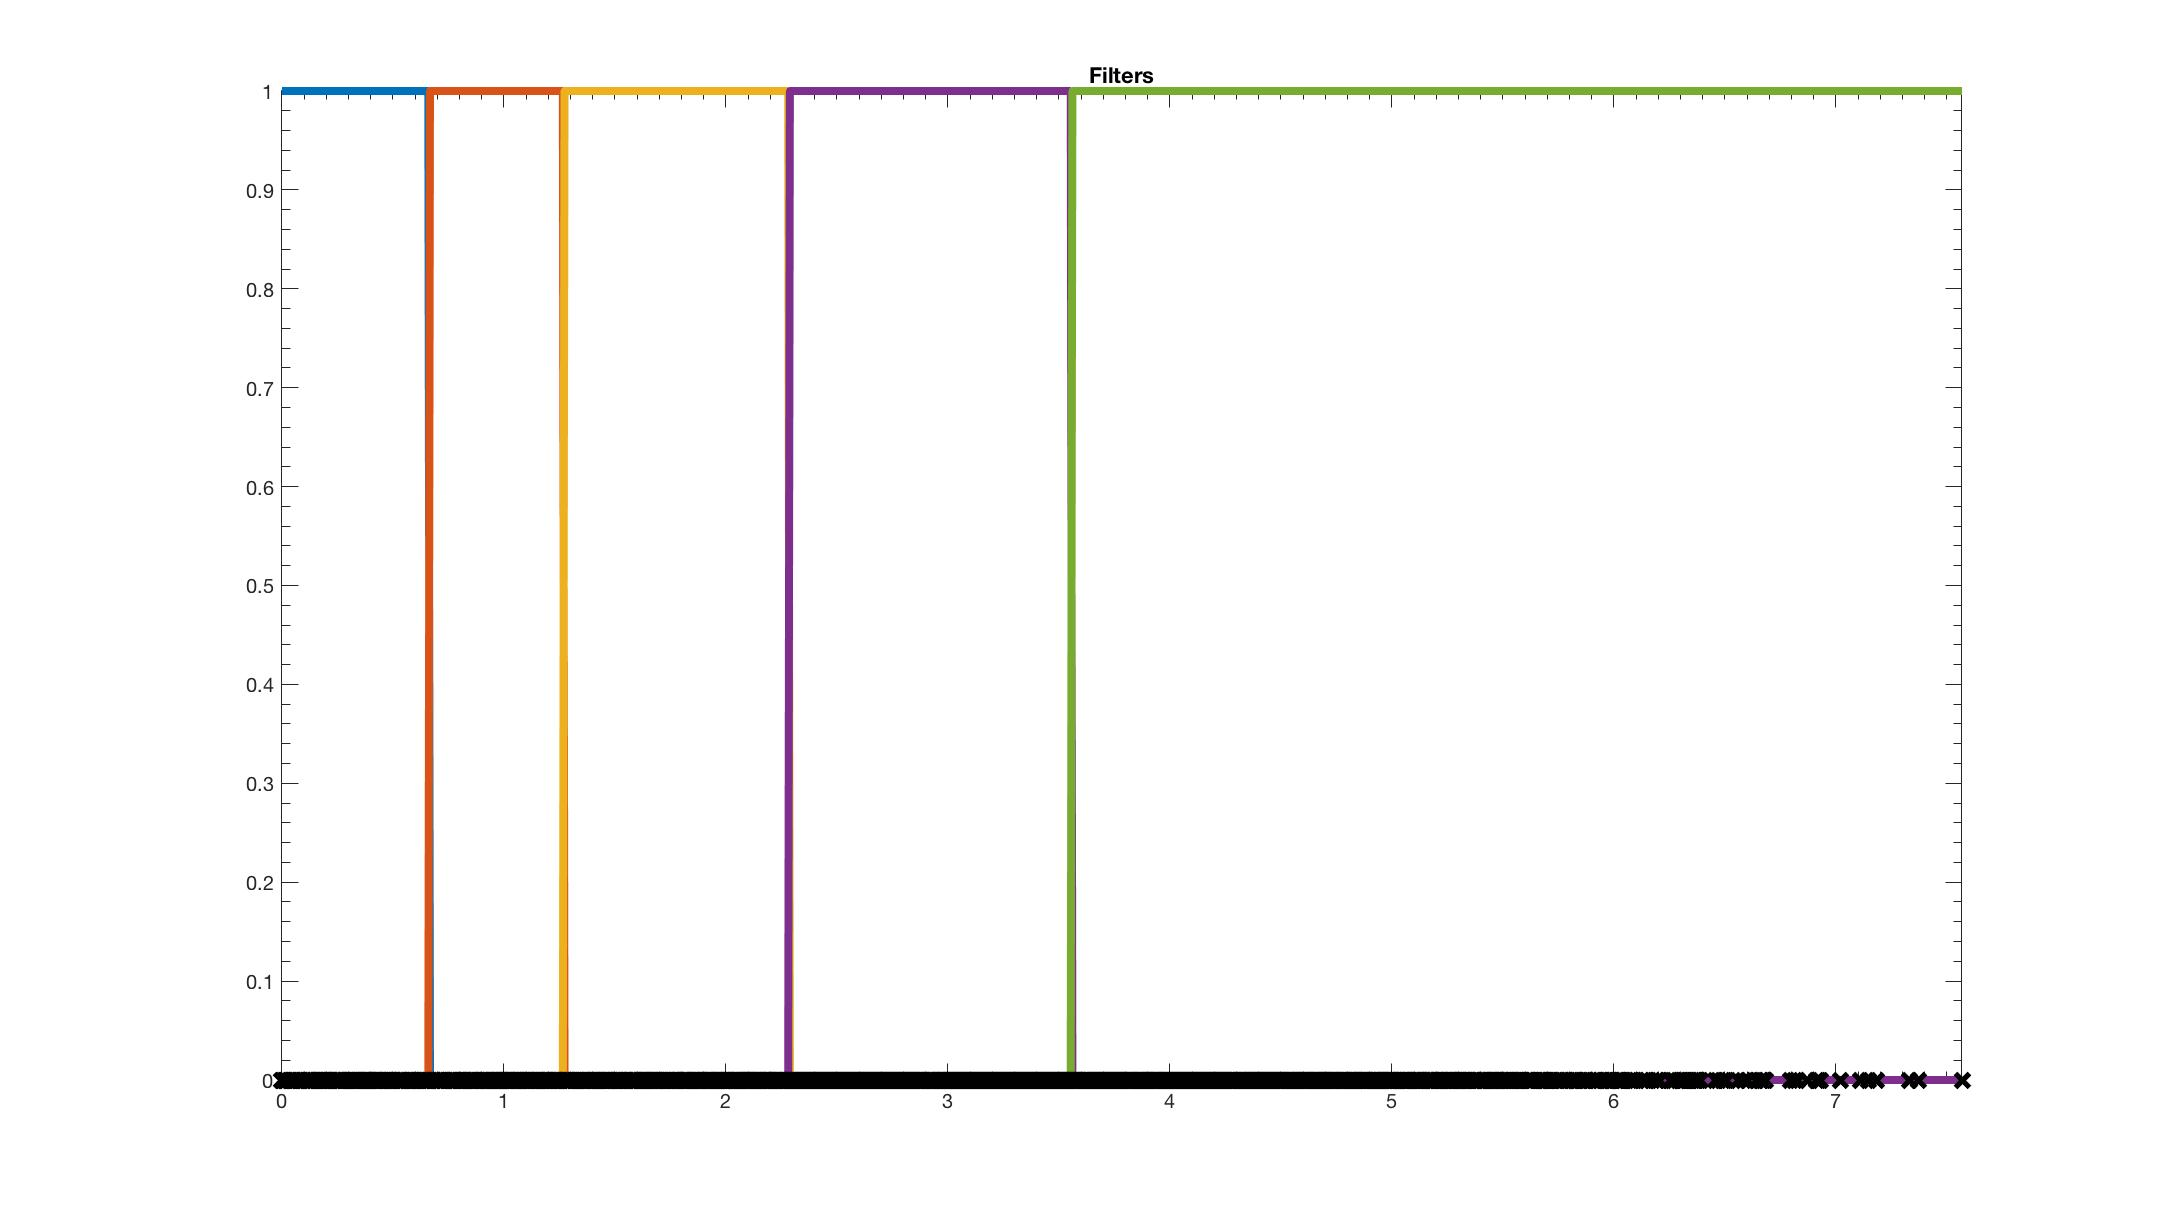
\includegraphics[width = 5cm]{filter_bank_1}
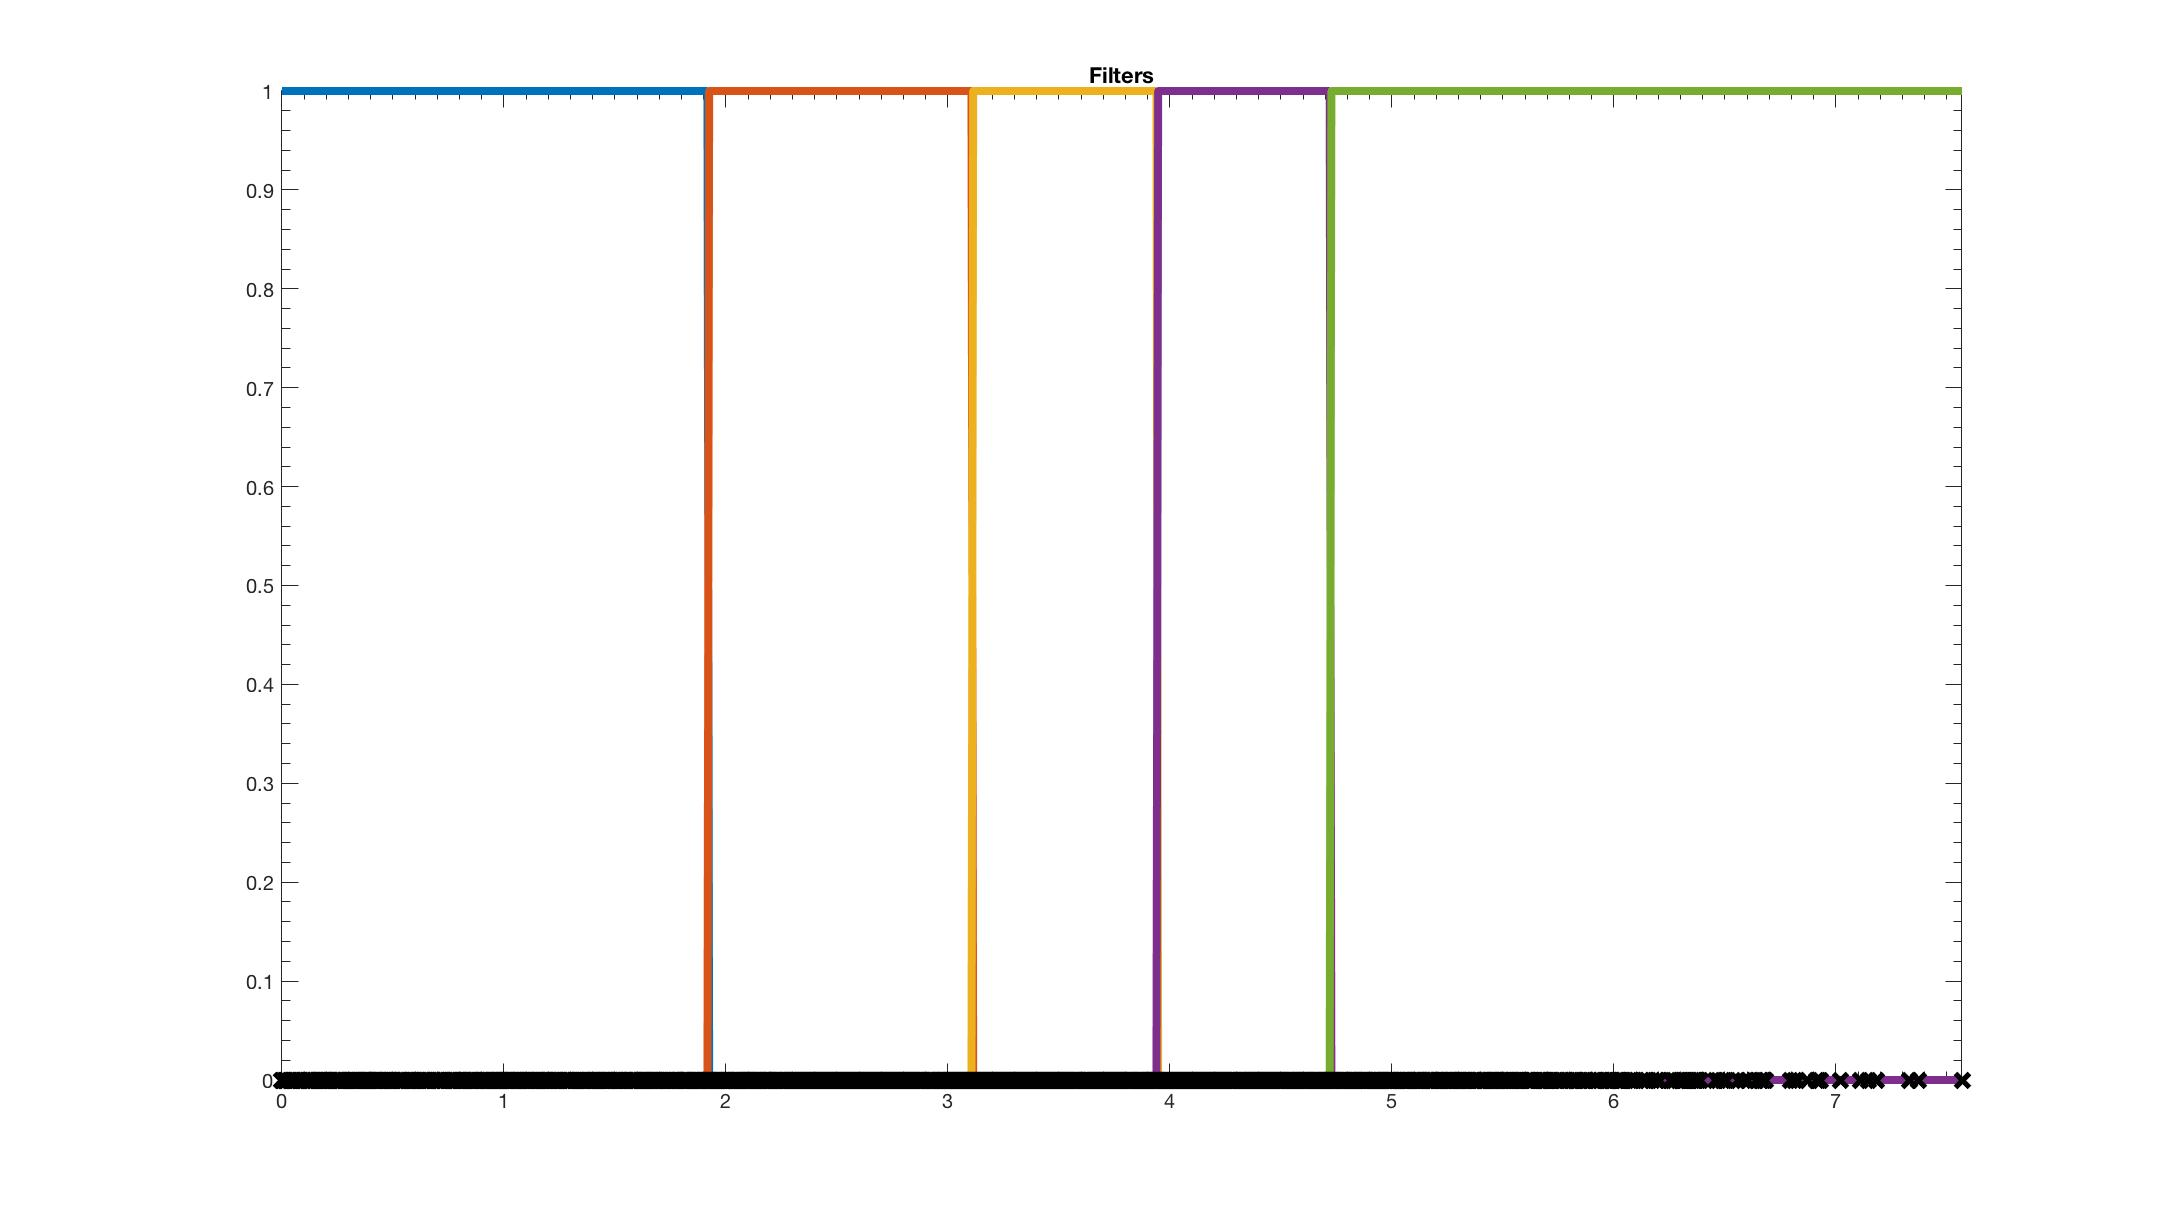
\includegraphics[width = 5cm]{filter_bank_2}

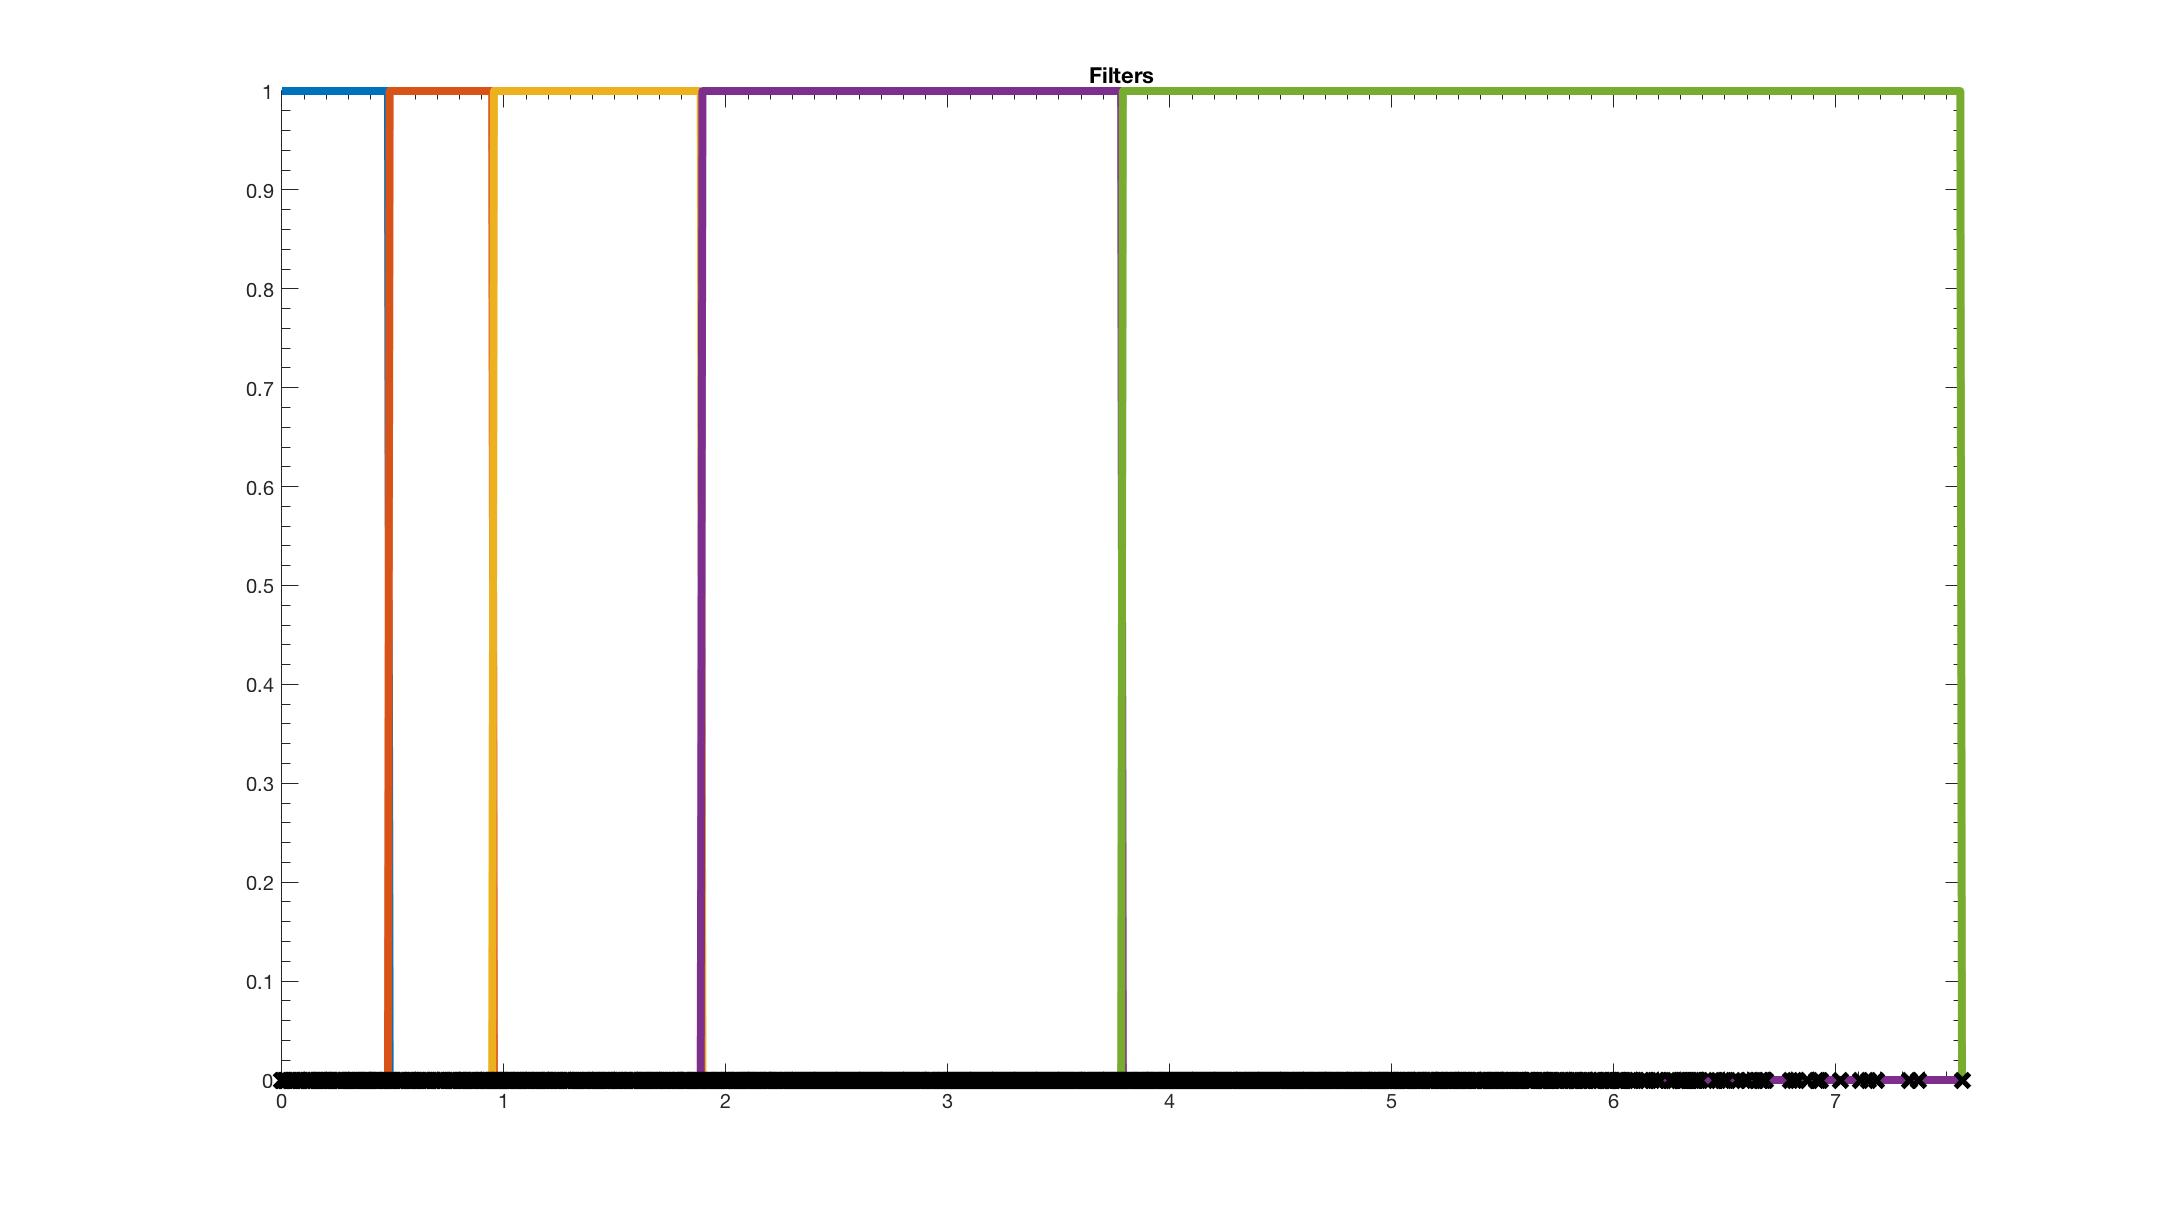
\includegraphics[width = 5cm]{filter_bank_4}
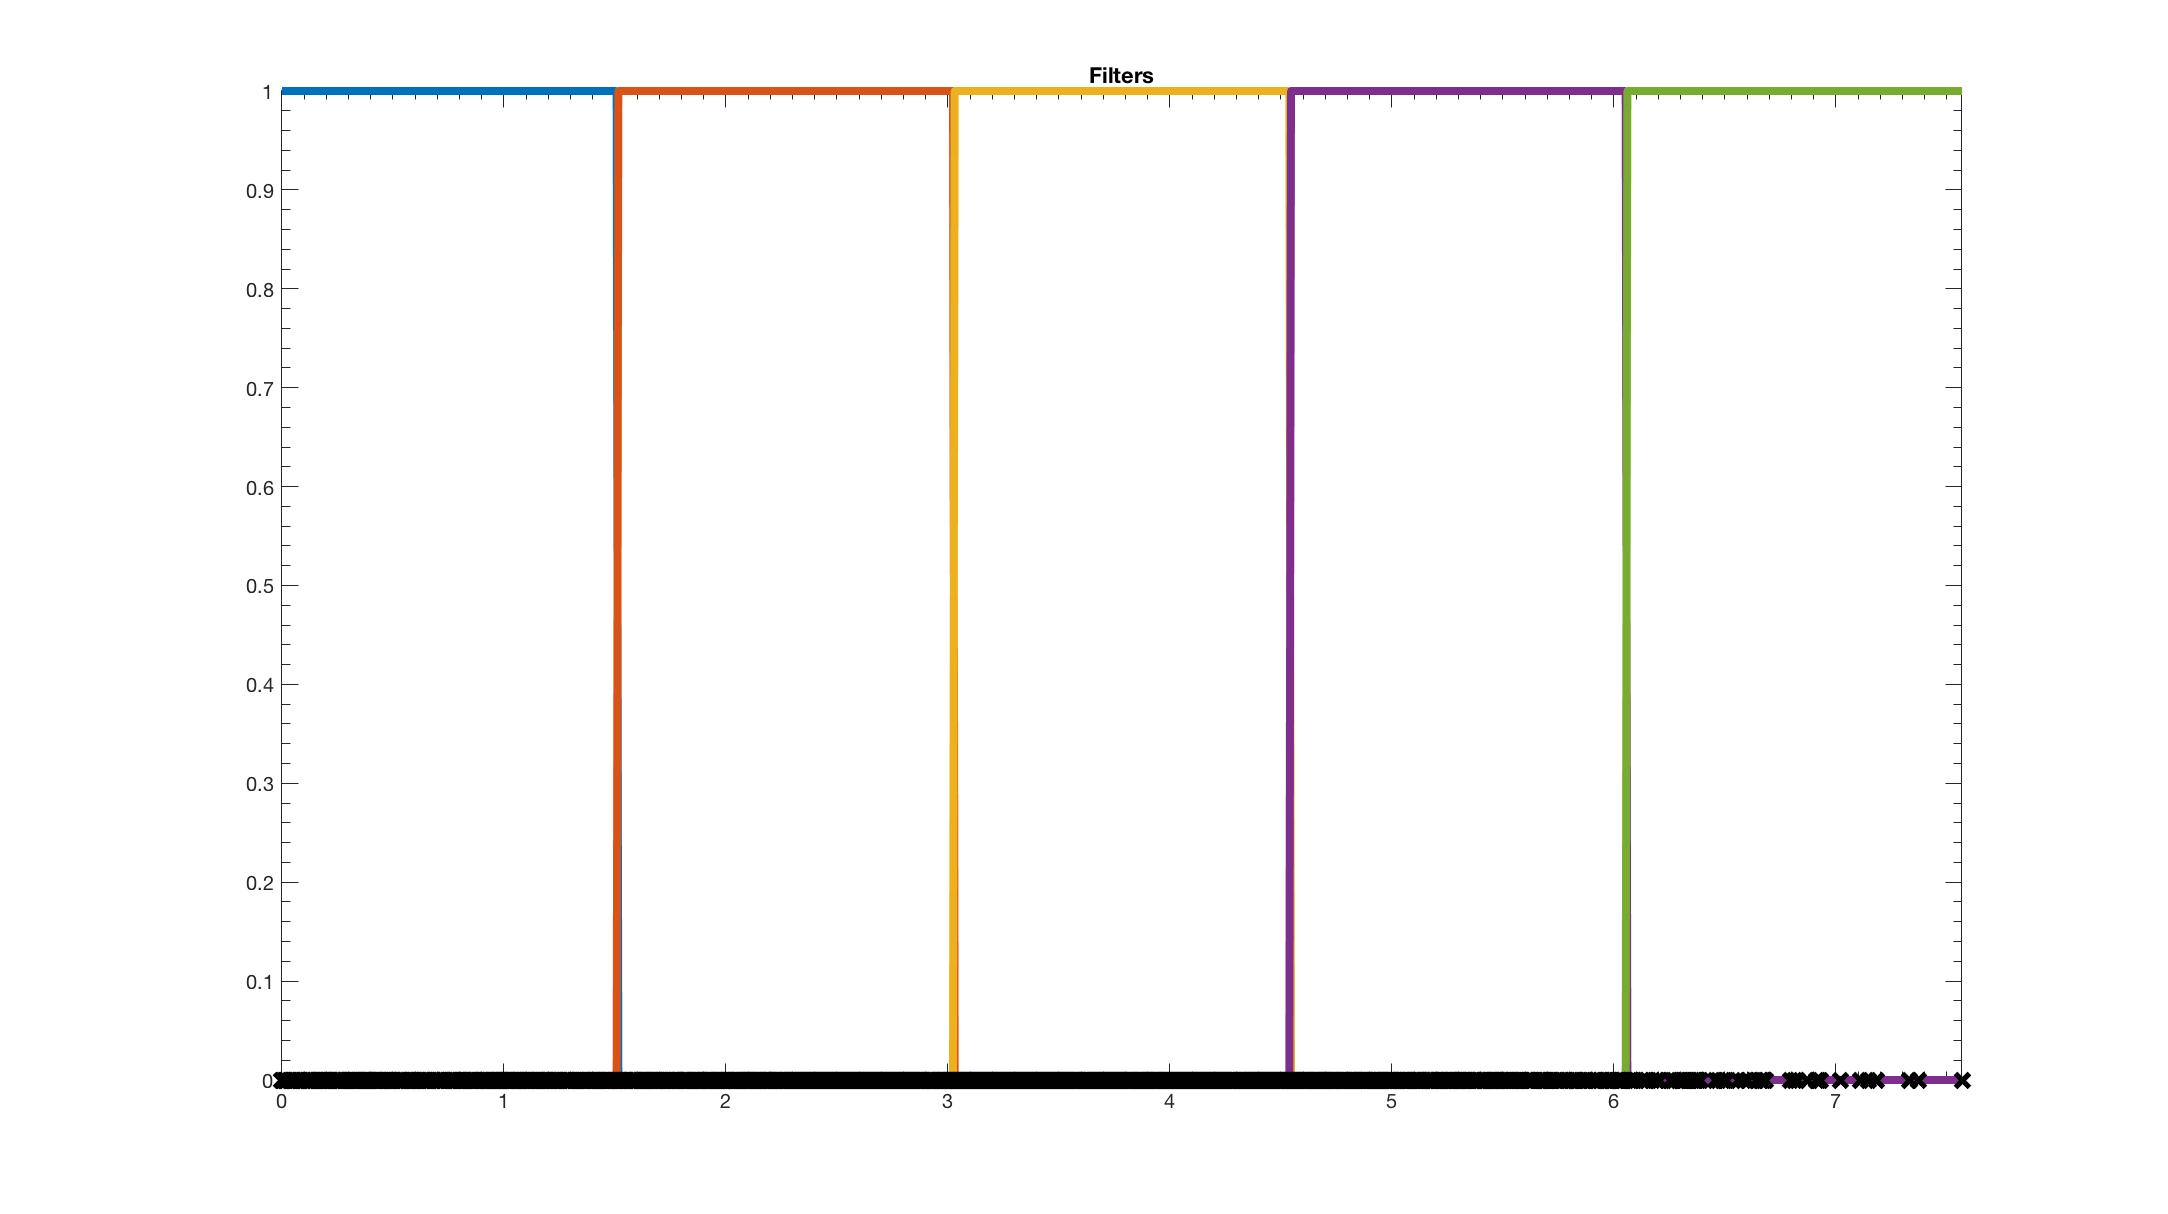
\includegraphics[width = 5cm]{filter_bank_3}


\caption{(a) is a spectrum-adapted and logarithmic spaced filter bank of 5 filters. Notice that this filter bank takes the density of Laplacian eigenvalues into account. The 4th filter covers half of the eigenvalues, the 3rd filter covers 1/4 of the eigenvalues, and each of the first two filters covers 1/8 of the eigenvalues.(b) stands for a spectrum-adapted but evenly spaced filter bank. Each of the five filters covers approximately the same number of eigenvalues. (c) and (d) are not spectrum-adapted. Notice that in this case the band ends only depend on the width of the spectrum.}
\end{figure}
\fi


\section{Non-Uniform Sampling and Reconstruction}


In this section, we select the dowmsampling sets using the non-uniform random sampling method and reconstruction the original signal from samples based on the the decoder derived from the sampling distribution. This method is first studied in \cite{random sampling} only for bandlimited signals. We extend this idea to all $\R$-concentrated signal models.

First, we need to determine the number of samples needed for each band in order to ensure critically sampling and perfect reconstruction. It has been shown in \cite{} \cite{} that any signal whose graph Fourier transform has exactly $k$ non-zero coefficients can be perfectly recovered from samples of that signal on $k$ appropriately selected vertices. That is, the number of samples needed equals the number of eigenvalues covered in the band. We use the spectral density function estimated in the previous section to approximate the number of eigenvalues in each band.

The goal of the non-uniform random sampling method is to minimizes the graph weighted coherence by imposing a sampling distribution on graph vertices. Graph weighted coherence is a quantity that measures of the localization of some Fourier modes on the nodes of the graph.The probability of node $i$ being selected is $p_i\propto ||U_{\R}^T\delta_i||_2$, which characterizes how much energy of $\delta_i$ is concentrated on the Fourier modes covered in $U_{\R}$. When this quantity is large, we would want high probability of selecting this node since there exists $\R$-concentrated signals whose energy is solely concentrated at the $i$th node. Including this node in our sample will increase our chance of perfect reconstruction later.

\begin{thm}[\cite{puy}, Theorem 3.2]
Consider any graph $\G = \{\V, \E, W\}$ with its Laplacian $\La = U\Lambda U^*$. Notice that $\La$ is real, symmetric and positive semi-definite and thus the columns of U are orthonormal and its eigenvalues are non-negative. We propose the following sampling procedure:

\begin{enumerate}

\item Sampling Distribution. Let $\R \subseteq \{0,1,\cdots, n-1\}$. Define $\bm{p} \in \RR^n$ as the sampling distribution on vertices $\{1,2, \cdots n\}$  such that 

\[\bm{p_i} = \frac{||U^T_\R\bm{\delta_i}||^2_2}{|\R|} \text{, for } i = 1,2 ,\cdots, n. \tag{1}\]  
The sampling distribution $\bm{p}$ minimizes the graph weighted coherence. We associate the matrix $P = \text{diag}(\bm{p}) \in \RR^{n\times n}$.

\item Subsampling Matrix. Let $\Omega = \{\omega_1, \omega_2, \cdots, \omega_m\}$ be the subset of nodes drew independently from the set $\{1,2,\cdots n\}$ according to the sampling distribution $\bm{p}$. Define $M$ as the random subsampling matrix with the sampling distribution $\bm{p}$ such that

\[M_{ij} = 
\begin{cases} 
      1 & \text{ if } j = \omega_{i}\\
      0 & \text{otherwise}
   \end{cases}
\tag{2}\] 

for all $i \in \{1,2,\cdots,m\}$ and $j \in \{1,2,\cdots, n\}$.

\end{enumerate}

\medskip

From the $m$ samples obtained using the sampling method above, we can reconstruction all $\R$-concentrated signals accurately by solving the optimization problem 
\[\underset{\bm{f} \in \text{span}(\UR)}{\text{min}}\vert\vert P^{-1/2}_\Omega (M\bm{f}-\bm{y})\vert\vert_2, \tag{3}\] 
which estimates signal $\bm{f} \in \RR^n$ from $\bm{y} \in \RR^m$. 

Let $\epsilon, \delta \in (0,1)$. Let $\bm{f^*}$ be the solution of the problem (3). With probability at lease $1-\epsilon$, the following holds for all $\bm{f}\in \text{span}(U_{\R})$ and all $\bm{n}\in \RR^m: $

\[||x^* - x||_2 \leq \frac{2}{\sqrt{m(1-\delta)} ||P_{\Omega}^{-1/2} \bm{n}||_2} \tag{4}\]
provided that \[m \geq \frac{3}{\delta^2}\vv^k_{\bm{p}}\log(\frac{2k}{\epsilon}). \tag{5} \]

\end{thm}




{\color{blue}
\section{Illustrative Examples II: Approximate Calculations}
\begin{itemize}
\item Make sure to have some very large examples and show computation times
\end{itemize}
}







\end{document}